\chapter{物理信息-门控循环单元(PI-GRU)流变学本构方程建模研究}

\section{引言}
上一章节通过GRU网络对流变数据进行时序建模,但是单纯的GRU网络属于纯数据驱动的黑箱模型,缺乏物理约束,在复杂模型和真实工况下,训练难度较高。本章节在GRU的基础上,引入物理信息约束,构建物理信息-门控循环单元(Physical Information-Gated Recurrent Unit,PI-GRU)模型。该模型以GRU为基础结构,并在损失函数中引入本构方程残差损失项,旨在利用GRU的门控机制捕捉黏弹性本构方程中的时间依赖性特征,同时确保模型符合物理约束,从而增强其泛化能力。

本章节首先通过数值模拟方法生成非线性的Giesekus模型数据,之后使用PI-GRU模型进行建模,并与其他模型进行对比,验证PI-GRU模型在复杂的非线性本构关系建模中的有效性。之后本章使用一类黏弹性聚合物的真实流变学实验数据进行PI-GRU训练和测试,验证PI-GRU模型在真实工况下的有效性。

\section{PI-GRU建模原理}
\subsection{Giesekus模型模拟数据}
Giesekus模型的本构方程如公式\eqref{eq:giesekus}所示,迁移因子$\alpha$用于引入剪切稀化的强度。Giesekus模型模拟的为简单剪切流动,只在xy方向存在应变,应变张量$\boldsymbol{\gamma}$仅在$\gamma_{12}$分量上存在值。
本章首先使用NumPy库生成8个不同速度场协议的简单剪切流动速度数据,再使用公式\eqref{eq:giesekus-gammadot}对应生成应变速率张量数据,时间区间为[0,24],单个协议的模拟数据点为2000,生成形式为3*3应变速率张量矩阵,之后根据$\gamma_{t}=\dot{\gamma}_{t-1}\Delta t+\gamma_{t-1}$迭代计算应变张量。
\begin{equation}
  \begin{aligned}
    \dot{\gamma}_{ii} & = 2 v_{ii}(t)           \\
    \dot{\gamma}_{ij} & = v_{ij}(t) + v_{ji}(t)
  \end{aligned} \label{eq:giesekus-gammadot}
\end{equation}
随后设置迁移因子$\alpha$为0.8,其余松弛时间参数($\lambda_1$、$\lambda_2$)为1.0,使用Python的scipy.integrate.solve\_ivp函数(内置方法为Runge-Kutta法)对Giesekus模型的微分方程组进行求解计算,生成3*3应力张量矩阵,如公式\eqref{eq:sigma_bmatrix}所示。本章提取$\sigma_{12}$、$\sigma_{11}$、$\sigma_{22}$分量作为模拟实验数据,与对应的应变速率张量数据、计算后的应变张量数据一起通过Pandas库存入Excel文件,便于后续的模型训练。
\section{PI-GRU建模方法}
Giesekus模型数据单独划分6个交变应变协议为训练集和验证集,其中按照9:1比例划分为训练集和验证集。划分1个交变应变协议,1个线性应变协议为测试集。

ABE弹性体数据选取1组SAOS数据和1组LAOS数据作为测试集,其余数据按照9:1比例划分为训练集和验证集。
\section{PI-GRU建模结果}
本章模型为PI-GRU架构,损失函数由数据损失和物理约束损失共同组成:
\begin{equation}
  \mathcal{L}_{\text{total}} =
  \lambda_{\text{data}} \mathcal{L}_{\text{data}} +
  \lambda_{\text{ode}} \mathcal{L}_{\text{ode}} +
  \lambda_{\text{dae}} \mathcal{L}_{\text{dae}}+
  \mathcal{L}_{L_{2}}
\end{equation}

\begin{equation}
  \mathcal{L}_{\text{data}} = \frac{1}{N} \sum_{i=1}^N
  \|\hat{\bm{\sigma}}_i - \bm{\sigma}_i^{\text{real}}\|_F^2
  \quad
\end{equation}

\begin{equation}
  \mathcal{L}_{\text{ode}} = \frac{1}{T-1} \sum_{t=1}^{T-1}
  \|\hat{\bm{\sigma}}_{t+1} - \Bigl[
    \hat{\bm{\sigma}}_t + \Delta t \cdot
    f_{\text{constitutive}}(\hat{\bm{\sigma}}_t, \dot{\gamma}_t)
    \Bigr] \|_F^2
  \quad
\end{equation}

\begin{equation}
  \mathcal{L}_{\text{dae}} = \frac{1}{T} \sum_{t=1}^T \Biggl(
  \underbrace{\|\hat{\bm{\sigma}}_t - \hat{\bm{\sigma}}_t^\top\|_F^2}_{\text{对称性约束}}
  \Biggr)
\end{equation}
\begin{equation}
  \mathcal{L}_{L_{2}} = \lambda \sum_{i} w_i^2
\end{equation}
其中数据损失$\mathcal{L}_{\text{data}}$通过MSE计算,目的是确保模型的预测结果与数值模拟数据尽可能接近,这是监督学习的基础,直接拟合数据,也是最重要和最基本的损失项。物理损失分为ODE损失$\mathcal{L}_{\text{ode}}$和对称损失$\mathcal{L}_{\text{dae}}$,物理损失确保模型的预测遵循本构方程描述的物理规律。这里的本构方程在模拟数值训练时为构建模拟数据的原方程,在真实实验数据(ABE弹性体数据)时为最小二乘法拟合的Maxwell方程。这部分损失是为了将物理知识融入模型,增强模型的泛化能力,抑制过拟合。
\section{PI-GRU建模分析}
作为真实实验数据测试的ABE弹性体的数据测试,本文选取一组SAOS数据和一组LAOS数据作为测试集,通过其他不同振幅的动态流变学数据训练,预测未知的振幅的应力应变Lissajous曲线。按照上述实验步骤分别使用极端梯度提升树(XGBoost)、多层感知器(MLP)、物理信息-多层感知器(PI-MLP)、物理信息-门控循环单元(PI-GRU)四种模型进行测试,绘制不同算法下的测试比对曲线。
% Giesekus模型建模
\subsection{Giesekus模型建模}
\subsubsection{数值模拟数据}
\begin{figure}[htbp]
  \centering
  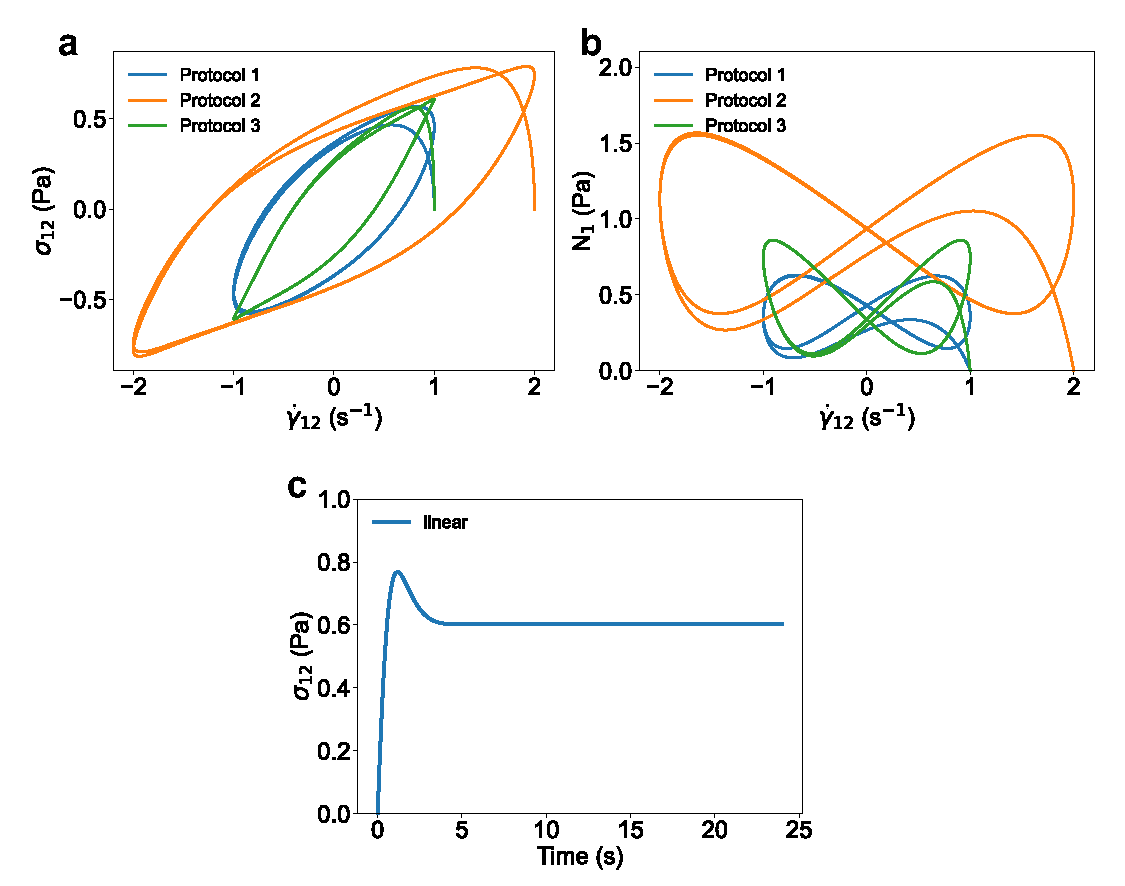
\includegraphics[width=0.8\textwidth]{Fig/giesekus-moni.pdf}
  \FigureBicaption{\label{giesekus_moni}Giesekus模型模拟数据:(a)不同交变应变协议的应力-应变率Lissajous曲线;(b)不同交变应变协议的第一法向应力差-应变率Lissajous曲线;(c)线性应变协议下的应力-时间曲线}{Giesekus model simulation data: (a) Lissajous curves of stress-strain rate for different oscillatory shear protocols; (b) Lissajous curves of first normal stress difference-strain rate for different oscillatory shear protocols; (c) Stress-time curve under linear strain protocol}
\end{figure}
本节通过Python的微分方程求解库来模拟Giesekus模型,模拟结果如图\ref{giesekus_moni}。

图\ref{giesekus_moni}展示了部分模拟数据,主要展示不同应变振幅下,本构关系从线性本构到非线性的转变。图\ref{giesekus_moni}(a)展示了不同交变应变协议的应力-应变率Lissajous曲线,Protocol 1为小振幅振荡剪切(SAOS)的模拟曲线,呈现椭圆状的滞后环,随着振幅增加,Protocol 2和 Protocol 3呈现非线性特征的扭曲和不对称,这是大振幅振荡剪切(LAOS)的拟合曲线。图\ref{giesekus_moni}(b)展示了不同交变应变协议的第一法向应力差(N$_1$)-应变率Lissajous曲线,随着振幅增加呈现不对称扭曲,曲线形状符合Giesekus模型假设\cite{lennonScientificMachineLearning2023a}。

图\ref{giesekus_moni}(c)为线性应变协议下的应力-时间曲线,曲线先随着应变加载攀升,存在明显峰值后回落,后趋于稳定。这可能是因为在屈服点之前,材料主要表现出弹性行为,应力随着应变的增加而线性增长。当应力达到峰值时,材料开始发生塑性变形,内部结构发生不可逆的变化,峰值之后,材料的内部结构开始重新组织,形成新的平衡状态,这种重组过程通常伴随着应力的下降与重新平衡。综上,线性协议的曲线符合Giesekus模型对于大剪切应变下材料应力响应的假设,可以用于后续实验。

\subsubsection{交变协议预测交变协议效果验证}
为了评估 GRU 算法在 Giesekus 模型本构方程数据预测中的有效性,本节采用交变应变协议生成的数据作为训练集与测试集,分别运用 GRU 和 DNN 进行模型训练,并在测试集上开展验证工作,测试结果如图 \ref{giesekus_sin}、图 \ref{giesekus-sin-metrics} 所示。

图 \ref{giesekus_sin}(a-c)分别为两种算法构建的预测模型所预测的剪切应力($\sigma_{12}$)的 Lissajous 曲线、时间-应力曲线以及残差图,(d- f)则对应预测的第一法向应力差(N$_{1}$)的Lissajous曲线、时间- 应力曲线与残差图。

从图a和图b可以观察到,GRU算法预测的$\sigma_{12}$值与真实值高度接近,曲线拟合效果理想,而DNN算法在部分区域的预测值存在较大偏差。图 c 的残差图进一步显示,GRU算法预测值与真实值的残差紧密围绕 0 刻度线,呈无序离散分布;相比之下,DNN算法预测值与真实值的残差呈现出明显的曲线规律及周期性特征,且与0刻度线的偏离程度较大,残差分布区间显著宽于GRU部分。残差图的结果有力地表明,GRU成功地学习到了训练数据中的各类特征及复杂的非线性关系,不存在明显的周期性规律,整体残差较小;而DNN存在未能充分学习特征的问题,拟合效果欠佳,未能精准捕捉训练数据的特征。

对于图d、图e和图f所展示的N$_{1}$预测效果,其与$\sigma_{12}$的结果呈现出相似性,即GRU的预测性能优于DNN。进一步对比GRU预测的N$_{1}$值和 $\sigma_{12}$值,发现$\sigma_{12}$值的预测效果更为优异,这可能归因于 $\sigma_{12}$与输入的剪切速率特征 $\dot{\gamma_{12}}$ 之间的函数关系相对简单,且更契合时间叠加原理,从而使得GRU能够更有效地捕捉其时间依赖性及内在联系。这部分的模型结果与Doi-Edwards模型结果类似,对于第一法向应力差(N$_1$),目前的GRU模型存在进一步改进的空间。
\begin{figure}[htbp]
  \centering
  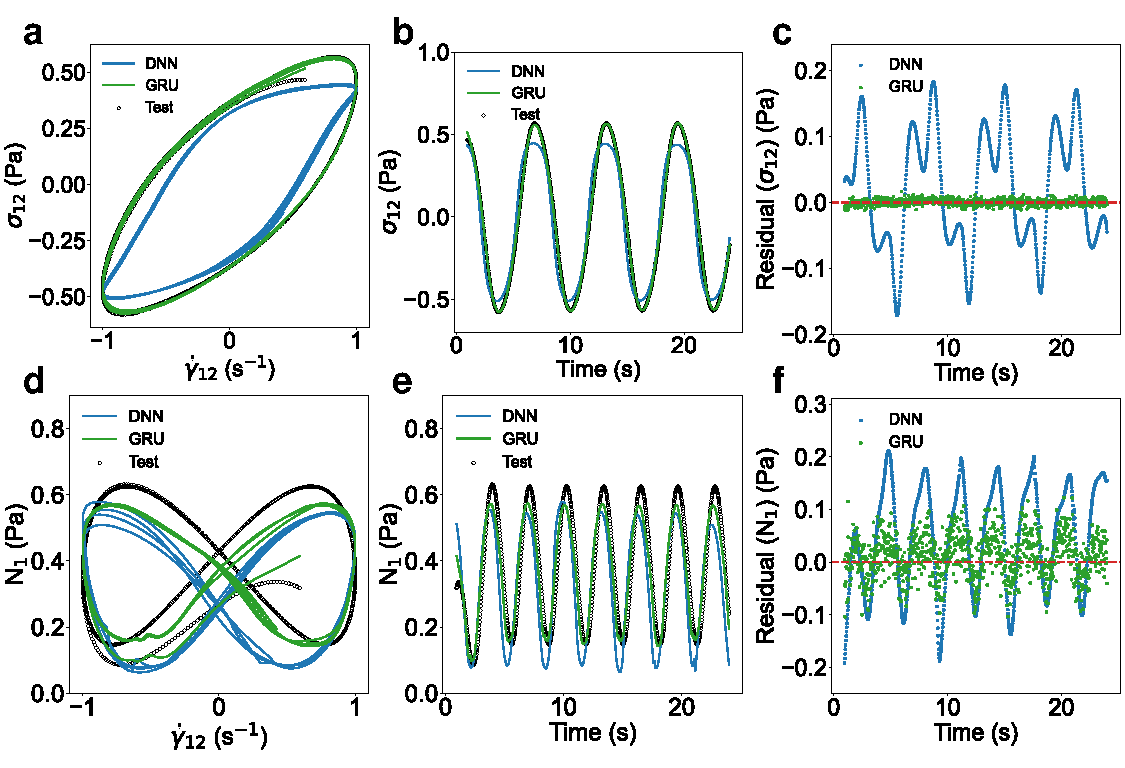
\includegraphics[width=0.8\textwidth]{Fig/giesekus_sin.pdf}
  \FigureBicaption{\label{giesekus_sin}GRU算法和DNN算法在Giesekus模型交变协议测试集上的预测效果对比示意图:(a)GRU和DNN在测试集上的预测值与真实值的剪切应力-应变率Lissajous曲线;(b)GRU和DNN在测试集上的剪切应力-时间曲线;(c)GRU和DNN在测试集上的剪切应力预测值残差图;(d)GRU和DNN在测试集上的预测值与真实值的第一法向应力差-应变率Lissajous曲线;(e)GRU和DNN在测试集上的第一法向应力差-时间曲线;(f)GRU和DNN在测试集上的第一法向应力差预测值残差图}{Comparison schematic of the prediction performance of the GRU algorithm and the DNN algorithm on the Giesekus model oscillatory protocol test set: (a) Shear stress-strain rate Lissajous curves of predicted vs. true values for GRU and DNN on test set; (b) Shear stress-time curves for GRU and DNN on test set; (c) Residual plots of shear stress predicted values for GRU and DNN on test set; (d) First normal stress difference-strain rate Lissajous curves of predicted vs. true values for GRU and DNN on test set; (e) First normal stress difference-time curves for GRU and DNN on test set; (f) Residual plots of first normal stress difference predicted values for GRU and DNN on test set}
\end{figure}
在本节中,进一步对两种算法在 $\sigma_{12}$ 和 N$_{1}$ 上的预测效果进行了定量分析,相关指标如图 \ref{giesekus-sin-metrics} 所示。
在 R$^2$指标方面,GRU 在 $\sigma_{12}$ 和 N$_{1}$ 的预测中均优于 DNN。此外,对于同一种算法,$\sigma_{12}$ 的 R$^2$ 值高于 N$_{1}$,例如GRU算法下$\sigma_{12}$的R$^2$值达到0.981,但是对应的N$_{1}$ 的 R$^2$ 值仅达到0.857。
在MAE指标方面,DNN的$\sigma_{12}$和N$_{1}$的MAE值分别为0.079和0.197,均显著高于GRU的0.004和0.051。而在$\sigma_{12}$上,GRU的MAE值为DNN的约二十分之一,对应地,在N$_1$上,GRU的MAE值为DNN的约四分之一。这说明GRU相比DNN的算法领先在$\sigma_{12}$上更为显著。
MAPE值的结果表明相同的结论,DNN预测结果的$\sigma_{12}$和N$_1$分别为112.5\% 和76.81\%,预测结果较差,而GRU的结果为2.68\% 和 15.44\%,预测效果显著优于DNN,且GRU相比DNN在$\sigma_{12}$的优化效果优于N$_1$,这与MAE的结论一致。
最后,从图 \ref{giesekus_sin}(d)可以看出,GRU在此项任务上的训练时间为1156 s,是DNN训练时间的5倍左右,符合其高计算成本的预期。
\begin{figure}[htbp]
  \centering
  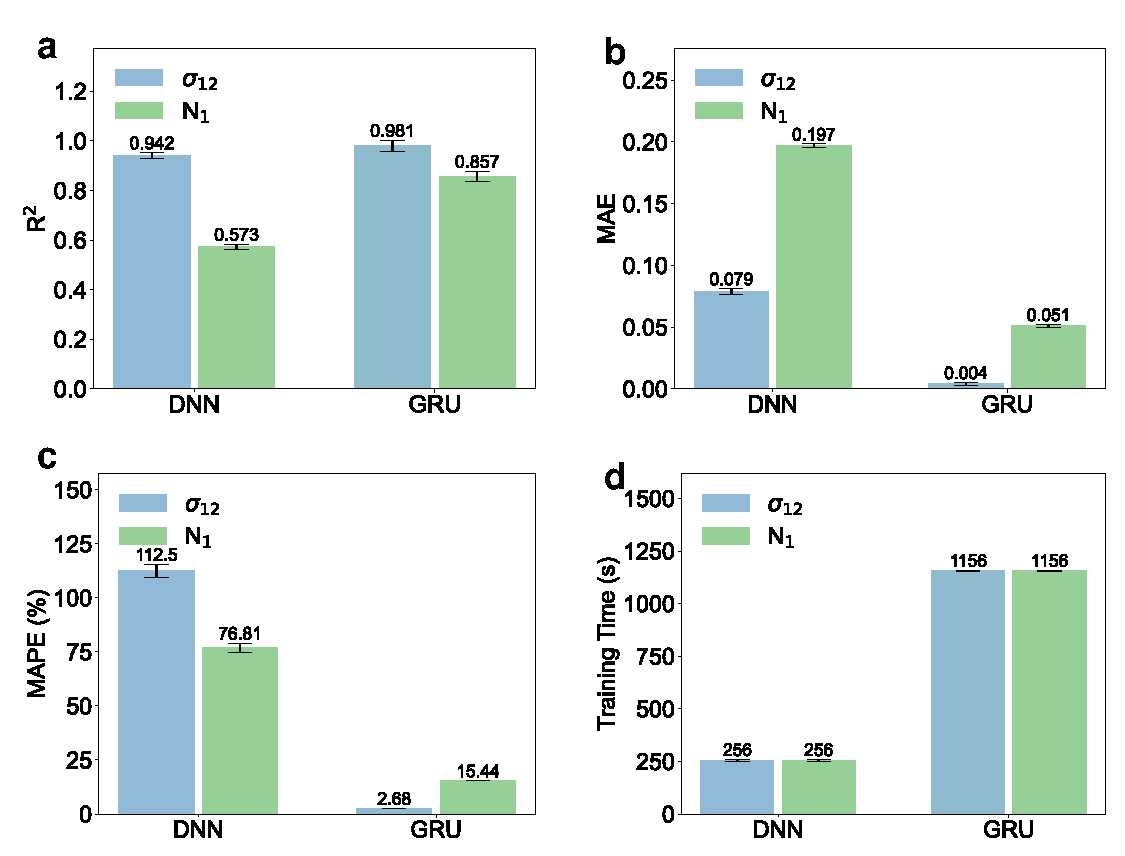
\includegraphics[width=0.8\textwidth]{Fig/giesekus-sin-metrics.pdf}
  \FigureBicaption{\label{giesekus-sin-metrics}GRU算法和DNN算法在Giesekus模型交变协议测试集上的预测效果对比示意图:(a)GRU和DNN在测试集上的R$^2$指标图;(b)GRU和DNN在测试集上的MAE指标图;(c)GRU和DNN在测试集上的MAPE指标图;(d)GRU和DNN在测试集上的训练时间指标图}{Comparison schematic of the prediction performance of the GRU algorithm and the DNN algorithm on the Giesekus model oscillatory protocol test set: (a) R$^2$ metric plots on the test set for GRU and DNN; (b) MAE metric plots on the test set for GRU and DNN; (c) MAPE metric plots on the test set for GRU and DNN; (d) Training Time metric plots on the test set for GRU and DNN}
\end{figure}
根据综合分析结果,当训练数据和测试数据均为交变应变时,GRU算法相比DNN能够更好地学习到Giesekus模型数据的内在特征。本节中,我们使用了SAOS和LAOS结合的训练数据,以探究模型对非线性黏弹性的学习能力。结果显示,GRU算法很好地完成了任务,成功捕捉了Giesekus模型模拟数据中的复杂非线性关系。综合来看,GRU算法在处理Giesekus模型的非线性黏弹性数据时表现出了显著的优越性,为后续研究提供了新的视角。

% Giesekus模型交变预测线性协议效果验证
\subsubsection{交变协议预测线性协议效果验证}
\begin{figure}[htbp]
  \centering
  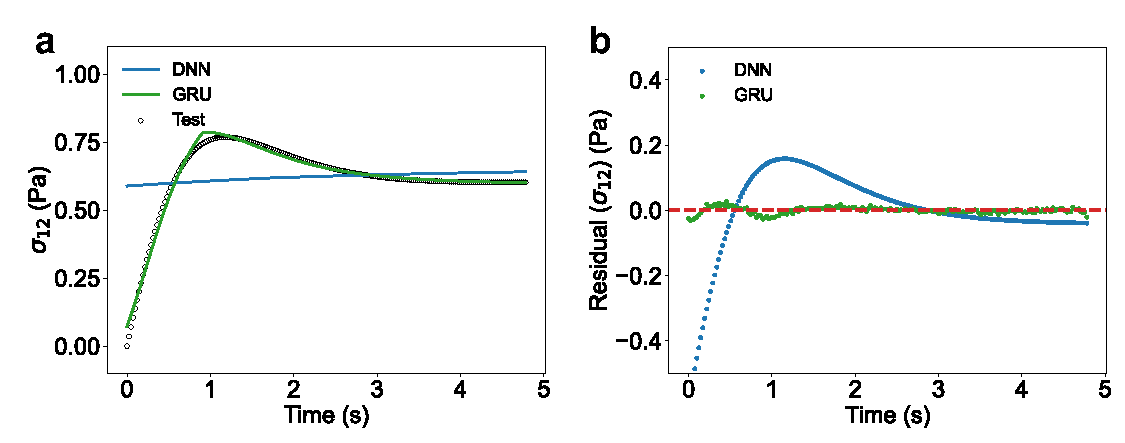
\includegraphics[width=0.8\textwidth]{Fig/giesekus-linear.pdf}
  \FigureBicaption{\label{giesekus-linear}GRU算法和DNN算法在Giesekus模型交变协议预测线性协议测试集上的预测效果对比示意图:(a)GRU和DNN在测试集上的时间-应力曲线;(b)GRU和DNN在测试集上的残差图}{Comparison schematic of the prediction performance of the GRU algorithm and the DNN algorithm on the Giesekus model oscillatory protocol predicting linear protocol test set: (a) Time-stress curves for GRU and DNN on test set; (b) Residual plots for GRU and DNN on test set}
\end{figure}
\begin{figure}[htbp]
  \centering
  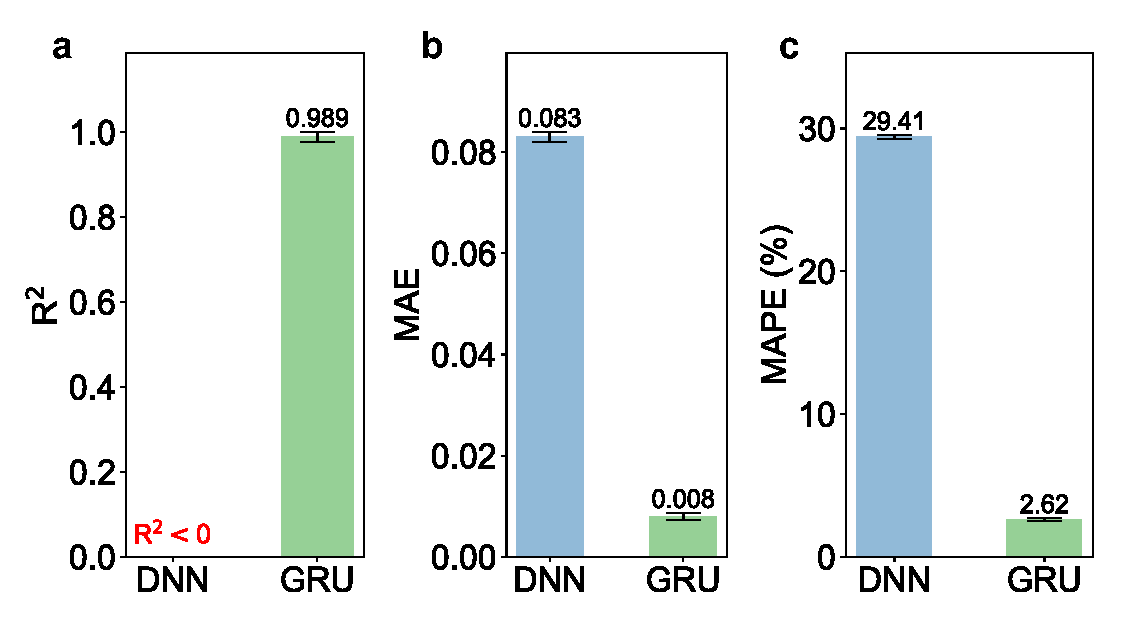
\includegraphics[width=0.8\textwidth]{Fig/giesekus-linear-metrics.pdf}
  \FigureBicaption{\label{giesekus-linear-metrics}GRU算法和DNN算法在Giesekus模型交变协议预测线性协议测试集上的预测效果对比示意图:(a)GRU和DNN在测试集上的R$^2$指标图;(b)GRU和DNN在测试集上的MAE指标图;(c)GRU和DNN在测试集上的MAPE指标图}{Comparison schematic of the prediction performance of the GRU algorithm and the DNN algorithm on the Giesekus model oscillatory protocol predicting linear protocol test set: (a) R$^2$ metric plots on the test set for GRU and DNN; (b) MAE metric plots on the test set for GRU and DNN; (c) MAPE metric plots on the test set for GRU and DNN}
\end{figure}
为了检验GRU算法在不同形式的应变历史下对Giesekus模型的泛化预测能力,本节采用交变应变协议生成的数据作为训练集,线性应变协议生成的数据作为测试集。分别使用GRU和DNN进行模型训练,并在测试集上进行验证,验证结果如图 \ref{giesekus-linear} 和图 \ref{giesekus-linear-metrics} 所示。

图\ref{giesekus-linear}(a)为两种不同算法预测模型在测试集上的真实值-预测值曲线,图中可以看到GRU算法的预测值的曲线与真实值曲线接近,仅在1-2 s之间存在小部分突出偏差,而DNN算法的预测值曲线完全没有拟合到曲线特征。图\ref{giesekus-linear}(b)展示了两种算法在测试集上的残差图。从图中可以明显看出,DNN算法的预测值与真实值之间的残差整体呈现出较为清晰的曲线趋势,存在明显的峰值。图中结果表明DNN完全没有捕捉到训练数据中的关键特征,导致其在测试集上的表现很差。与之形成鲜明对比的是,GRU 算法的残差图呈现出无序分布的特征,残差点均匀地分布贴近在 0 刻度线两侧。这一现象表明,GRU 能够更有效地学习数据中的关键特征,从而实现更小的预测偏差。结合真实值与预测值的曲线分析以及残差图的观察,可以分析出GRU在此项任务的预测性能优于DNN。


具体如图\ref{giesekus-linear-metrics} 所示。从图\ref{giesekus-linear-metrics}(a)可以清晰地观察到,GRU 算法的 R$^2$值高达 0.989,这一结果有力地表明了 GRU 在预测任务中的出色表现。与之形成鲜明对比的是,DNN算法的R$^2$值小于 0,这表明 DNN 并未有效学习到相关特征。进一步分析图\ref{giesekus-linear-metrics}(b-c),可以发现 GRU 预测结果的平均绝对误差(MAE)值为 0.008,而 DNN的 MAE 值则高达 0.083。这表明GRU 在绝对误差方面的表现仅为DNN的十分之一,优势极为明显。此外,GRU 预测结果的平均绝对百分比误差(MAPE)值为2.62\%,而DNN 的 MAPE 值则为 29.41\%。这些定量数据充分证明了 GRU 的预测结果误差小于 DNN,从而进一步证实了 GRU 在该任务上的预测泛化能力更强。
在两种算法的训练时间对比方面,与上一节中交变协议预测交变协议的情况相同,具体可参考图 \ref{giesekus-sin-metrics}(d)所示。

\subsubsection{不同时间步的预测效果对比}
\begin{figure}[htbp]
  \centering
  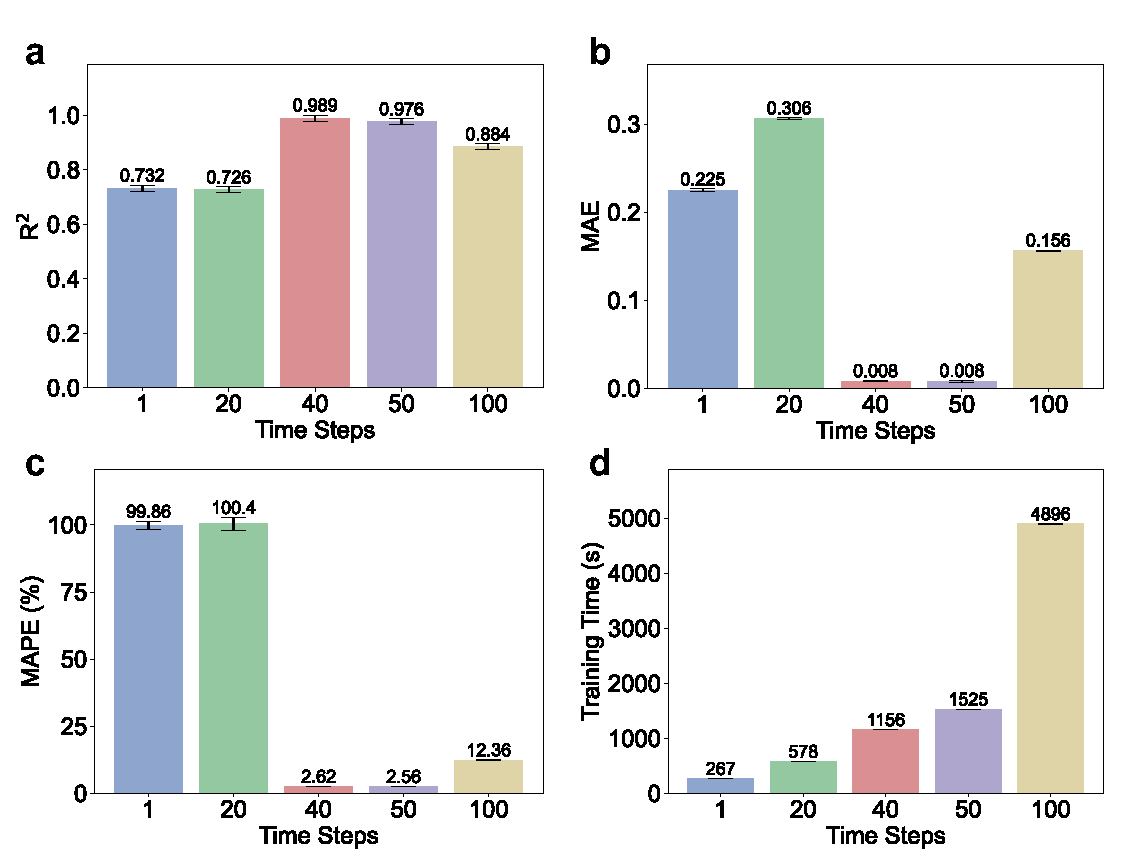
\includegraphics[width=0.8\textwidth]{Fig/giesekus-timesteps-metrics.pdf}
  \FigureBicaption{\label{giesekus-timesteps-metrics}GRU算法和DNN算法在Giesekus模型不同时间步长下的预测指标对比图:(a)GRU和DNN在不同时间步下的R$^2$指标图;(b)GRU和DNN在不同时间步下的MAE指标图;(c)GRU和DNN在不同时间步下的MAPE指标图;(d)GRU和DNN在不同时间步下的训练时间指标图}{Comparison schematic of the prediction performance of the GRU algorithm and the DNN algorithm under different time steps of the Giesekus model: (a) R$^2$ metric plots under different time steps for GRU and DNN; (b) MAE metric plots under different time steps for GRU and DNN; (c) MAPE metric plots under different time steps for GRU and DNN; (d) Training Time metric plots under different time steps for GRU and DNN}
\end{figure}
为了探究在Giesekus模型上GRU算法的最佳时间步,本节研究了不同时间步下训练的模型在测试集上的预测效果,如图\ref{giesekus-timesteps-metrics}所示。由图可见,预测模型R$^2$值在时间步小于40时为0.7左右,当时间步为40时为0.969,时间步进一步增加,R$^2$开始下降。MAE值在时间步为40相比20时从0.306调跃减少至0.008,进一步增加时间步,MAE值不再显著改变,直到时间步为100,MAE值回升至0.156,显现过拟合趋势。MAPE值变化趋势与MAE值类似,在时间步为40左右跳跃减少,随后直到100步开始回升。从训练时间来看,随着时间步增加,训练时间单调增加,这一点与预期一致。




\subsection{真实数据集实验}
为了验证我们的PI-GRU模型在真实数据集上的表现,本文选取了ABE弹性体数据集,训练数据集为SAOS和LAOS的混合数据集,测试集分为SAOS和LAOS数据两类以验证模型在线性区间和非线性区间的预测效果。由图\ref{fgr:real-data-differstrain}可知,PI-GRU模型在SAOS测试集上相比对比的XGBoost模型、多层感知器(MLP)模型、PI-MLP模型(该模型构建参考Mahmoudabadbozchelou)\cite{mahmoudabadbozchelouDatadrivenPhysicsinformedConstitutive2021}具有最佳的预测效果,预测指标(图\ref{fgr:real-data-differstrain-saos-metrics})中MAPE值仅为3.33\%,属于优秀泛化范畴,相比PI-MLP模型的14.9\%下降了11.57\%,在训练时间成本上,PI-GRU模型为1070s相比PI-MLP模型(789s)仅增加了281s。
\begin{figure}
  \centering
  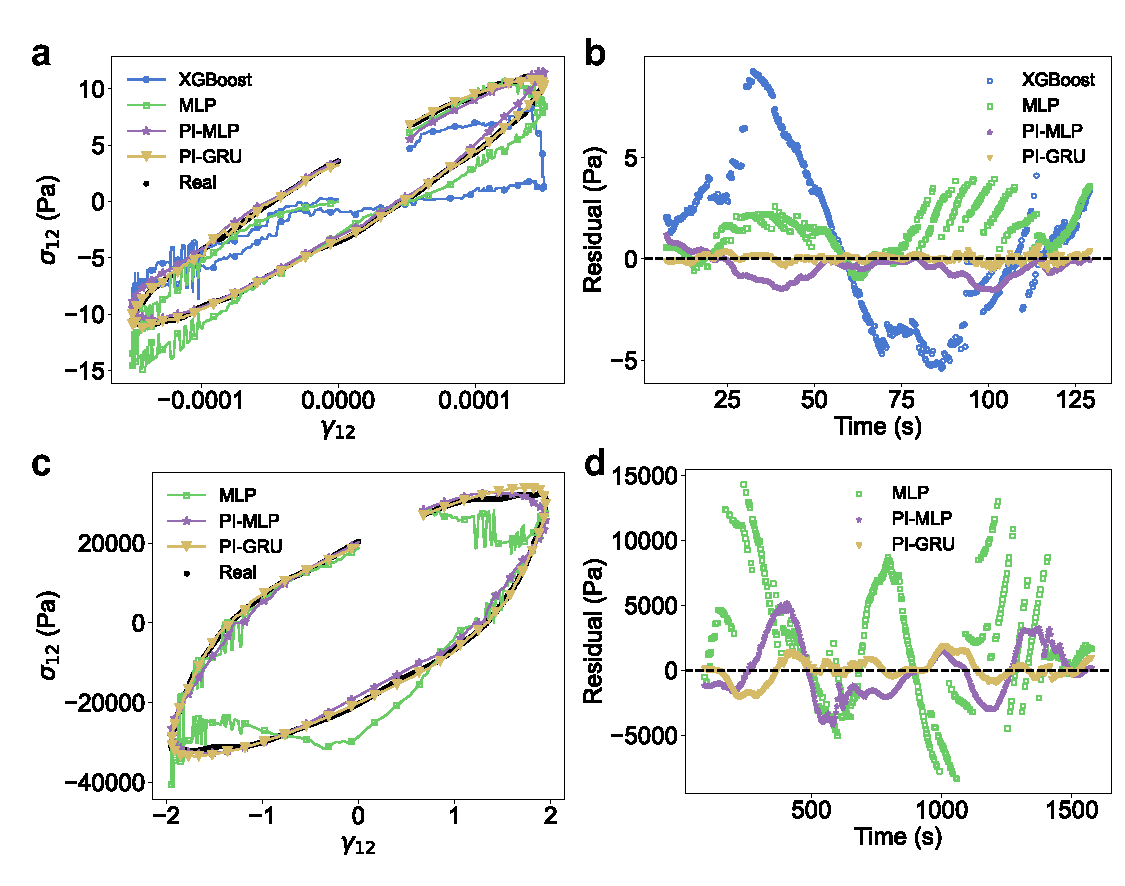
\includegraphics[width=0.8\textwidth]{Fig/real-data-differstrain.pdf} % 此处填写图片名
  \FigureBicaption{\label{fgr:real-data-differstrain}ABE弹性体的Lissajous曲线在不同算法上的预测效果:(a)小振幅振荡剪切(SAOS)测试集真实值与模型预测值的Lissajous曲线对比;(b)小振幅振荡剪切(SAOS)测试集真实值与模型预测值的残差图;(c)大振幅振荡剪切(LAOS)测试集真实值与模型预测值的Lissajous曲线对比;(d)大振幅振荡剪切(LAOS)测试集真实值与模型预测值的残差图}{Prediction performance comparison of Lissajous curves for ABE elastomer using different algorithms: (a) Comparison of Lissajous curves between true values and model predictions on small-amplitude oscillatory shear (SAOS) test set; (b) Residual plot of true values and model predictions on SAOS test set; (c) Comparison of Lissajous curves between true values and model predictions on large-amplitude oscillatory shear (LAOS) test set; (d) Residual plot of true values and model predictions on LAOS test set}
\end{figure}
\begin{figure}
  \centering
  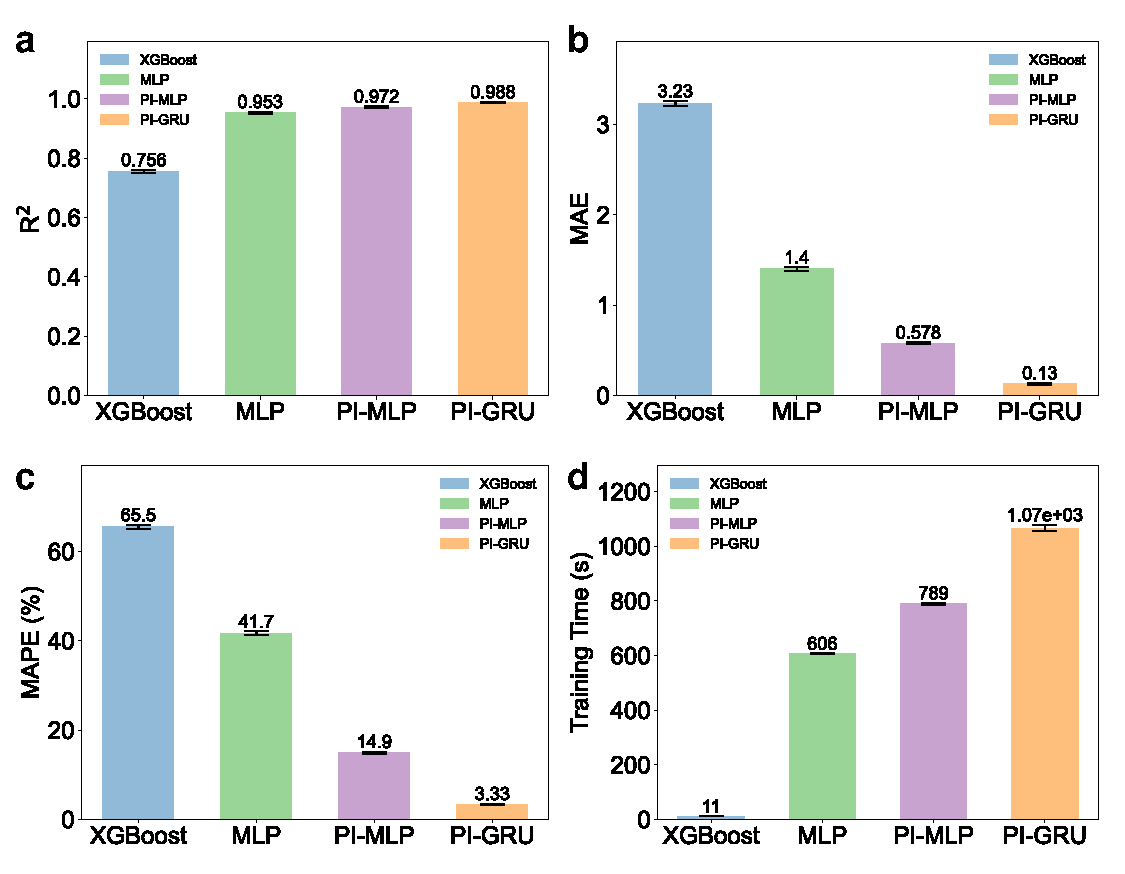
\includegraphics[width=0.8\textwidth]{Fig/real-data-differstrain-saos-metrics.pdf} % 此处填写图片名
  \FigureBicaption{\label{fgr:real-data-differstrain-saos-metrics}}{不同算法在ABE弹性体SAOS实验Lissajous曲线上的预测指标对比:(a)决定系数(R²),(b)平均绝对误差(MAE),(c)平均绝对百分比误差(MAPE),(d)计算训练时间}{Comparative Evaluation of Predictive Metrics for ABE Elastomer's Lissajous Curves in SAOS Experiments Across Algorithms: (a) Coefficient of Determination (R²), (b) Mean Absolute Error (MAE), (c) Mean Absolute Percentage Error (MAPE), (d) Computational Training Time}
\end{figure}

\begin{figure}
  \centering
  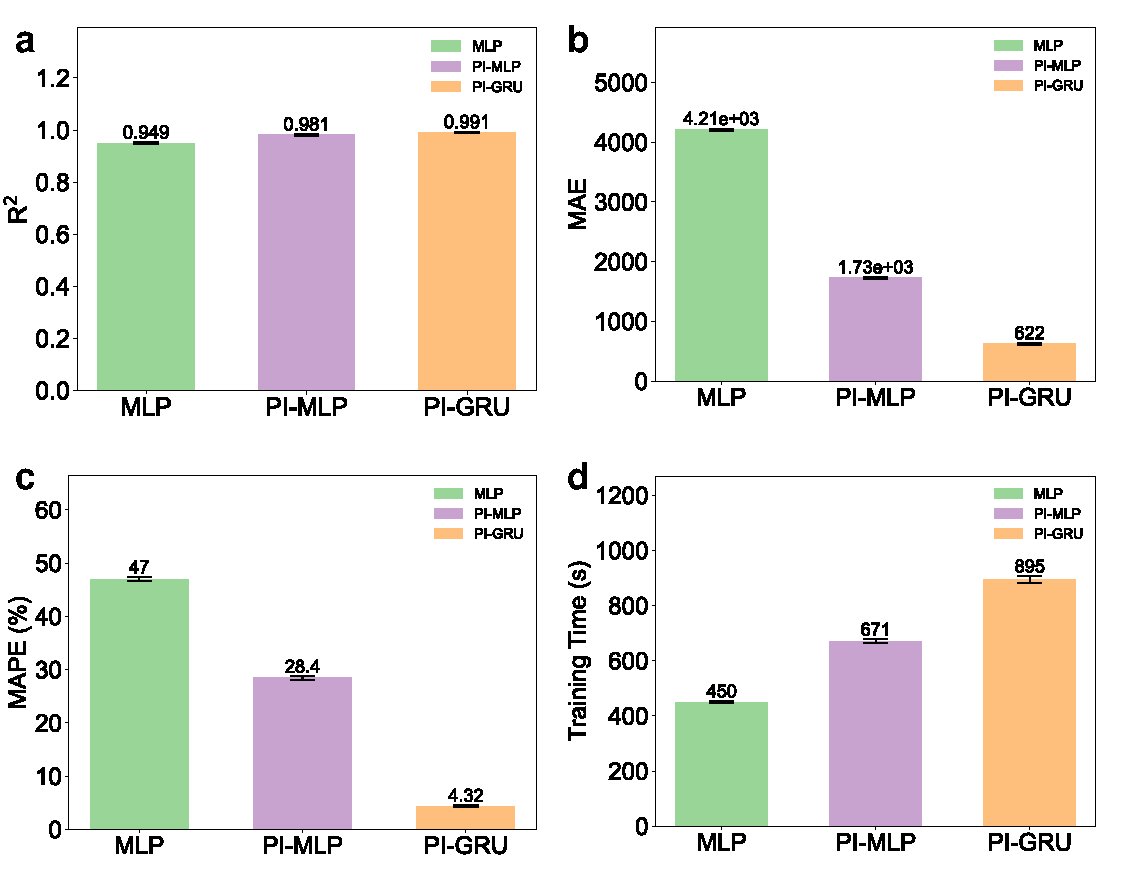
\includegraphics[width=0.8\textwidth]{Fig/real-data-differstrain-laos-metrics.pdf} % 此处填写图片名
  \FigureBicaption{\label{fgr:real-data-differstrain-laos-metrics}}{不同算法在ABE弹性体LAOS实验Lissajous曲线上的预测指标对比:(a)决定系数(R²),(b)平均绝对误差(MAE),(c)平均绝对百分比误差(MAPE),(d)计算训练时间}{Comparative Evaluation of Predictive Metrics for ABE Elastomer's Lissajous Curves in LAOS Experiments Across Algorithms: (a) Coefficient of Determination (R²), (b) Mean Absolute Error (MAE), (c) Mean Absolute Percentage Error (MAPE), (d) Computational Training Time}
\end{figure}
LAOS测试集上,如图\ref{fgr:real-data-differstrain}(c-d)所示,PI-GRU的表现大幅度领先对比模型,PI-GRU模型预测指标(图\ref{fgr:real-data-differstrain-laos-metrics})中MAPE值仅为4.32\%,相比PI-MLP模型的28.4\%下降了24.08\%,在训练时间成本上,PI-GRU模型为895s相比PI-MLP模型(671s)仅增加了224s。这一结果说明,PI-GRU模型在处理非线性黏弹性材料的流变学数据时,能够更好地捕捉到数据中的时间依赖性特征,这是因为门控单元可以自主决定是否记忆和遗忘信息,即对于每一个时间步的应变状态历史,门控单元自主给予不同的权重,从而更好地拟合非线性区应力历史叠加并非玻尔兹曼叠加原理的流变学数据,这一特性使得GRU结构相当于对黏弹性材料的历史依赖性做了特有的特征融合,这是作为前馈神经网络的MLP模型无法做到的。值得注意的是,在预测过程中,物理约束损失的本构方程形式为最简单的Maxwell模型(并未引入非线性点),然后就结果来看,PI-GRU模型依旧可以很好地泛化到非线性区间的LAOS数据,这是因为物理约束给予的是大致的物理规律符合,例如Oldroyd-B类模型(Giesekus、FENE-P、​LPTT)通过不同形式的非线性修正扩展了基础模型的适用范围,而GRU模型在Maxwell模型的物理约束下从另一种独特的形式修正扩展了基础模型。由于简单Maxwell模型的参数拟合非常简单,且本文的研究并不需要过分追求物理约束部分的本构方程的参数精确度,因此该模型可以低成本地扩展到其他不同的流变学实验体系。
\section{PI-GRU建模总结}
在Giesekus 模型的研究中,本章模拟了小振幅振荡剪切(SAOS)以及大振幅振荡剪切(LAOS)这两种不同的工况。实验结果表明,GRU 的建模效果优于 DNN,这有力地说明 GRU 所捕捉的时间依赖性,不仅仅局限于基于玻尔兹曼叠加原理的线性黏弹性的时间特性,还能够涵盖更为复杂的非线性关系,而Giesekus模型下GRU对第一法向应力差N$_1$的预测效果也比$\sigma_{12}$差。
为了进一步探究GRU在真实数据集上的表现,本章选取了ABE弹性体的流变学实验数据集进行验证。使用简答Maxwell模型作为物理约束残差方程,设计物理信息约束的门控循环单元(PI-GRU)。通过将PI-GRU模型与XGBoost、MLP以及PI-MLP等模型进行对比,结果显示PI-GRU模型在测试集上表现最佳。特别值得注意的是,即使在物理约束采用最简单的Maxwell模型的情况下,PI-GRU模型仍然能够很好地泛化到非线性区间的LAOS数据,这充分证明了该模型在处理复杂流变学数据时的优越性。